
\chapter{Návrh}\label{chap:design}

V~tejto kapitole predstavíme základný algoritmus a postupne sa budeme venovať jeho jednotlivým častiam. Budeme sa venovať metódam na zlepšenie úspešnosti klasifikátora a porovnáme rôzne prístupy. 
\bigskip

\section{Základný algoritmus}

Základný algoritmus (Obr. \ref{fig:base_alg}) vyzerá nasledovne: 
Najskôr sa získa obraz z webkamery. Ten sa potom spracuje a následne sa rozsegmentuje na jednotlivé pohybujúce sa objekty.
Každý z týchto segmentov sa predloží klasifikátoru, ktorý rozhodne, či daný segment je, alebo nie je ruka. Zo všetkých segmentov je vybratý ten, o ktorom si je klasifikátor najviac istý, že je ruka (a zároveň spĺňa danú hranicu). Z vybratého segmentu sa vypočíta bod, ktorý je braný ako pozícia ruky. Tento bod je pridaný do postupnosti bodov, o ktorých sa ďalej rozhodne, či tvoria niektoré gesto. Ak klasifikátor gesta detekuje nejaké gesto, vykoná sa príslušná akcia - simulácia stlačenia niektorej klávesy - a postupnosť sa vymaže. Ak sa dlhšiu dobu v obraze nevykonala žiadna zmena a klasifikátor gesta nezistil žiadne gesto, postupnosť sa tiež vymaže.

\begin{figure}[htp]
    \centering
%    \includegraphics[scale=1]{img/00/extern-drive-encryption.1.mps}
    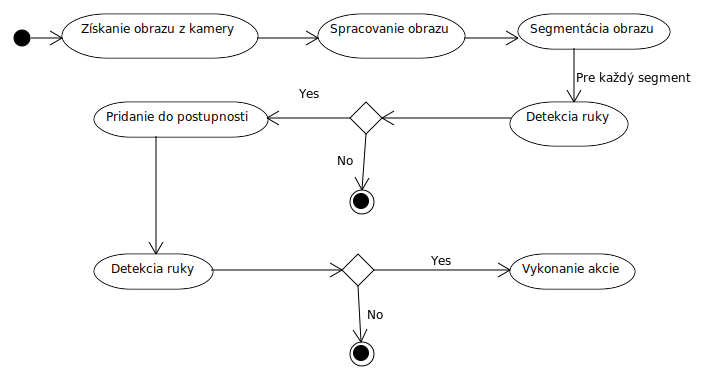
\includegraphics[width=\textwidth]{images/BaseAlgorithm}
%    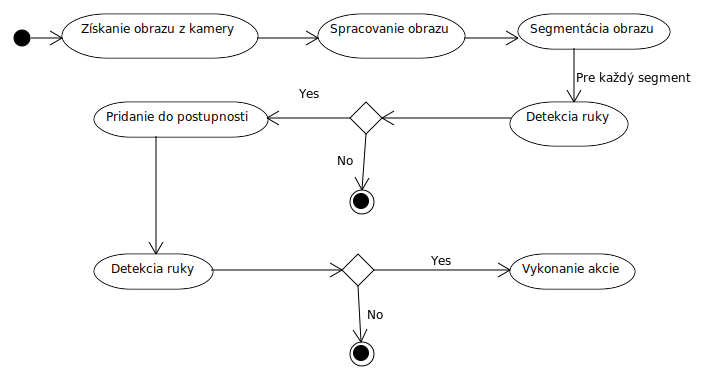
\includegraphics[scale=1]{images/BaseAlgorithm}
    \caption{Základný algoritmus}
    \label{fig:base_alg}
\end{figure}

\subsection{Predspracovanie a segmentácia}\label{chap:preprocess}

Základ pre predspracovanie a segmentáciu tvorí takzvaný \textbf{rozdielový obraz}. Rozdielový obraz je obraz, ktorý vznikne odčítaním 2 posebe idúcich čiernobielych obrázkov v absolútnej hodnote. Tento obraz obsahuje zmeny - pohybujúce sa objekty. Statické objekty sa tam teda nevyskytnú, čo nám umožní ich veľmi ľahko odfiltrovať. V tomto obraze sa vyskytnú obrysy pohybujúcich sa objektov, pretože ku zmenám dochádza najviac na hranách. Podľa rýchlosti pohybu môžu byť obrysy hrubšie, alebo tenšie. 
Našim cieľom je čo najlepšie zachytiť pohybujúcu sa ruku.

Dohodneme sa, že najmenšia zmena (žiadna) bude znázornená bielou a najväčšia čiernou. 

\subsubsection{Odfiltrovanie šumu}
Odfiltrovanie šumu zabezpečí hranica. Všetky pixle svetlejšie ako určitá konštanta, budú vykreslené bielou. Ideálna hranica je taká, ktorá potlačí šum, ale zachová čo najviac z ostatných zmien - čiže by mala byť najmenšia možná. Pohybujeme sa v odtieňoch šedej, čiže hodnoty $0\dots 255$. Praktické testy ukázali, že vhodnou hodnotou pre hranicu je 7.

\subsubsection{Rozpitie pixlov}

Kvôli segmentácii potrebujeme aby jednotlivé segmenty boli súvislé. Teda aby obrys ruky tvoril jeden celok.
Ľahko sa nám však môže stať, že obrys ruky je niekde prerušený - nedostatočná zmena, prípadne iné dôvody. Predpokladáme ale, že všetky časti jedného segmentu sú dostatočne blízko. Spojiť segmenty nám teda pomôže rozpitie pixlov. 

%TODO spravnu konštantu, spomenut rozlisenie
Z každého pixla spravíme štvorec s veľkosťou $11\times 11$.
Hodnota 11 pre stranu štvorca sa ukázala ako najvhodnejšia. 
Príliš veľké hodnoty spájajú aj časti, ktoré nepatria do toho istého segmentu, príliš malé zase nespoja časti, ktoré sú ďalej od seba.

\subsubsection{Segmentácia}\label{subsubsect:segment}
Rozpitý obrázok si teraz vieme predstaviť ako graf, pričom hrana je medzi každými 2 susediacimi pixlami (v štyroch smeroch). Segmentácia je vlastne len nájdenie komponentov v tomto grafe. Na to môžeme použiť napríklad prehľadávanie do šírky. Samozrejme musíme ešte nájsť opísaný obdĺžnik - stačí nájsť najľavejší, najpravejší, najvrchnejší a najspodnejší bod segmentu.

\subsection{Spracovanie segmentov}
Každý nájdený obdĺžnik sa naškáluje na veľkosť vstupu pre neurónovú sieť - v našom prípade $128\times 128$ - a normalizuje sa.

%Neural Net
\section{Návrh architektúry neurónovej siete}\label{chap:neuralnetarch}

V tejto kapitole si popíšeme rôzne architektúry sietí, ktoré sme vyskúšali a porovnáme ich vlastnosti a úspešnosť pri riešení problému rozpoznania ruky a vyberieme vhodnú architektúru, ktorú potom použijeme v našej aplikácii.

\subsection{Cieľ}

Našim cieľom je vytvoriť vhodnú architektúru neurónovej siete, ktorá bude rozhodovať o danom vstupe, či zodpovedá ruke alebo nie. Vyskúšame niekoľko typov architektúr, porovnáme ich a následne vyberieme najvhodnejšiu, ktorú potom použijeme. 

Neurónová sieť má rozdeliť vstupy do 2 tried - tie, ktoré zodpovedajú rukám a ostatné. Na to využijeme vo všetkých architektúrach jeden výstupný neurón.

\subsection{Trénovanie}

Na generovanie dát sme použili upravenú verziu našej aplikácie, ktorá umožňovala ukladanie vysegmentovaných obrázkov na disk. Aby sme dostali čo najrealistickejšie obrázky, potrebovali sme aby aplikácia išla takmer tak rýchlo ako pôvodná. Zápis na disk je však časovo náročná operácia, preto sme si obrázky ukladali do buffera a zapisovali dávkovo. Zapisovali sme čo najmenšie množstvo dát, preto sme dáta fourierovych transformácií\footnote{viď kapitola \ref{sect:metodyzlepseniaklasifikacie} } robili až dodatočne ďalšou aplikáciou.

Trénovanie dopredných sietí sme robili pomocou algoritmu \textit{Backpropagation} - algoritmu spätného šírenia chyby \cite{haykin1999neural} . Sieti sme postupne predkladali dáta s informáciou či sa jedná o ruku alebo nie. Pred každou epochou sme dáta náhodne preusporiadali. 

Pri rekurentných sieťach sme predkladali postupnosti dát, pričom sme zachovávali poradie obrázkov v postupnosti. Rekurentné vstupy sme updatli len v prípade, že sme detekovali ruku. Po každej postupnosti sme rekurentné vstupy resetli na 0. Takto simulujeme správanie siete v reálnej aplikácii.

Na trénovanie sme použili dáta fourierovych transformácií (viď \ref{sect:ft}). Množina dát obsahovala cca 800 vzorov, ktoré boli pri trénovaní rekurentnej neurónovej siete rozdelené do približne 70 postupností.

\subsection{Testovanie a vyhodnocovanie neurónových sietí}
Pri trénovaní sa snažíme minimalizovať kvadratickú chybu. Preto aj pri vyhodnocovaní úspešnosti sietí budeme používať túto veličinu.

Kvadratická chyba sa počita takto: $\frac{1}{2}(t-o)^2$, kde $t$ je cieľová hodnota a $o$ je výstup siete. V tabuľkách budeme uvádzať priemernú kvadratickú chybu, ktorú budeme počitať ako súčet všetkých kvadratických chýb deleno počet testovacích vstupov. 

Na testovanie sme mali množinu cca 650 vzorov (60 postupností), ktoré sme nepoužívali na trénovanie.

\subsection{Viac vrstvová dopredná neurónová sieť}

\textbf{Viac vrstvová dopredná neurónová sieť} (obr. \ref{fig:ffnn}) je neurónová sieť zložená z viacerých vrstiev neurónov, pričom signál sa šíri len zo spodnejšej vrstve na vyššiu. V našej implementácii siete sa ako vstup každého neurónu berie výstup každého neurónu z predošlej vrstvy. Prvá vrstva dostane pôvodný vstup. 

Experimentálne sme zistili, že dvojvrstvová sieť na tento problém stačí a tretia vrstva nepomáha.
% - 3vrstvovú sieť sa nám ani nepodarilo natrénovať 
V tabuľke \ref{tab:neuroncountcmp} je porovnanie úspešnosti na testovacích dátach a priemerná kvadratická chyba.

\begin{table}[h]
\catcode`\-=12 %kvoli babelu a pomlcke
\centering
\begin{tabular}{|l|c|c|c|c|c|}
\cline{2-5}
\multicolumn{1}{l}{} & \multicolumn{2}{|c|}{\textbf{Testovacia sada}} & \multicolumn{2}{c|}{\textbf{Trénovacia sada}} & \multicolumn{1}{l}{}\\ 
\hline
\textbf{Počet neurónov} & \textbf{úspešnosť} & \textbf{chyba} & \textbf{úspešnosť} & \textbf{chyba} & \textbf{čas} \\ \hline
40 & 81,11\% & 0,0818 & & &\\ \hline
45 & 85.55\% & 0,0643 & & &\\ \hline
50 & 85,19\% & 0,0667 & & &\\ \hline
60 & 85,19\% & 0,0634 & & &\\ 
\hline
\end{tabular}
\caption{Porovnanie úspešnosti NS pri rôznych počtoch neurónov}
\label{tab:neuroncountcmp}
\end{table}


\subsection{Viac vrstvová dopredná neurónová sieť - upravená verzia}

\begin{figure}[h]
  \begin{center}
    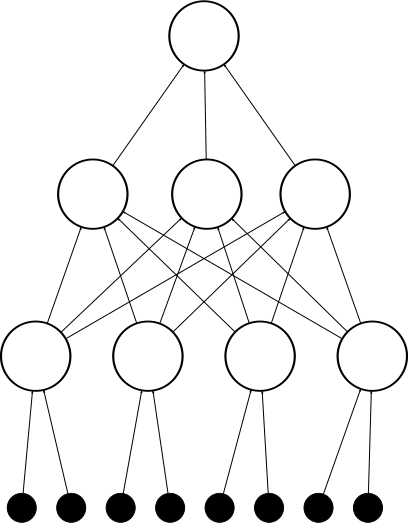
\includegraphics[width=0.3\textwidth]{images/dffnn}
  \end{center}
  \caption{Upravená dopredná neurónová sieť}
  \label{fig:dffnn}
\end{figure}


V upravenej verzii sme upravili spodnú vrstvu siete - tú, ktorá dostáva vstup. Vstup je rozdelený na 16 častí a ku každej časti je pridelených niekoľko neurónov. Každý neurón spracúva len vstupy z jeho časti (obr. \ref{fig:dffnn}). 

Jej výhodou je rýchlosť. Náš vstup má rozmer $128\times 128 = 16384$, čo nie je malé číslo. Rozdelíme ho na 16 častí s veľkosťou $32\times 32 = 1024$. Takto namiesto toho aby každý vstupný neurón počítal s 16384 vstupmi počíta len s 1024, čo je $16\times$ rýchlejšie. Skupina neurónov pridelená danej časti sa stará len o príznaky zo svojej časti a nie je ovplyvňovaná ostatnými časťami. 

Nevýhodou je to, že neuróny sú fixne pridelené na jednotlivé vstupy. V pôvodnej sieti si neuróny sami vyberali, ktoré časti vstupu sú pre nich najvýznamnejšie a mohli tak lepšie pokryť vstup.

\begin{table}[h]
\catcode`\-=12 %kvoli babelu a pomlcke
\centering
\begin{tabular}{|l|c|c|c|c|c|}
\cline{2-5}
\multicolumn{1}{l}{} & \multicolumn{2}{|c|}{\textbf{Testovacia sada}} & \multicolumn{2}{c|}{\textbf{Trénovacia sada}} & \multicolumn{1}{l}{}\\ 
\hline
\textbf{Počet neurónov} & \textbf{úspešnosť} & \textbf{chyba} & \textbf{úspešnosť} & \textbf{chyba} & \textbf{čas} \\ \hline
48; 12 & 83,33\% & 0,0745 & & &\\ \hline
112; 12 & 84,07\% & 0,0714 & & &\\
\hline
\end{tabular}
\caption{Porovnanie úspešnosti upravenej NS pri rôznych počtoch neurónov}
\label{tab:neuroncountcmp2}
\end{table}

Keď si porovnáme tabuľku \ref{tab:neuroncountcmp2} s tabuľkou \ref{tab:neuroncountcmp} zistíme, že rozdiel v úspešnosti nie je veľký. Preto sme sa rozhodli, že použijeme radšej túto architektúru. Trénovanie aj klasifikácia je značne rýchlejšia.
%TODO popisat aj pocty pouzitych neuronou 
%TODO trenovacie data do tabuliek

\subsection{Rekurentná neurónová sieť}

Architektúra našej rekurentnej neurónovej siete vychádza z upravenej doprednej neurónovej siete, s tým, že namiesto obyčajného neurónu používame v niektorej vrstve rekurentný neurón (obr. \ref{fig:recurentneuron}) viac v kapitole \ref{chap:rnn}.

\begin{table}[h]
\catcode`\-=12 %kvoli babelu a pomlcke
\centering
\begin{tabular}{|l|c|c|c|c|c|}
\cline{2-5}
\multicolumn{1}{l}{} & \multicolumn{2}{|c|}{\textbf{Testovacia sada}} & \multicolumn{2}{c|}{\textbf{Trénovacia sada}} & \multicolumn{1}{l}{}\\ 
\hline
\textbf{Rekurentná vrstva} & \textbf{úspešnosť} & \textbf{chyba} & \textbf{úspešnosť} & \textbf{chyba} & \textbf{čas} \\ \hline
spodná & 83,33\% & 0,0745 & & &\\ \hline
\end{tabular}
\caption{Porovnanie úspešnosti rekurentnej NS pri rôznom umiestnení rekurencie}
\label{tab:neuroncountcmp2}
\end{table}

%end NeuralNet

\section{Metódy na zlepšenie úspešnosti klasifikátora ruky}
\label{sect:metodyzlepseniaklasifikacie}

V tejto časti sa budeme zaoberať jednotlivými segmentami, ktoré budeme predkladať neurónovej sieti, aby nám povedala, či je to ruka, alebo nie.

\subsection{Normalizácia dát}
Ideálne vstupy pre neurónovú sieť sú z intervalu $<0,1>$. Pixle čiernobielych obrázkov majú hodnoty $\{0\dots 255\}$. Pri obrázkoch zvolíme pre farbu pozadia hodnotu 0 a pre objekt ostatné hodnoty. Z tohto dôvodu chceme, aby rozdiel v normalizovanej hodnote medzi 0 a 1 bol najväčší a postupne klesal. Preto sme za normalizačnú funkciu zvolili:

$$f(x)=\frac{1}{1+x}$$

Pre normalizáciu fourierovej transformácie sme zvolili tú istú funkciu. %TODO dôvod? 

\subsection{Pôvodný vs. rozdielový obrázok}
Nevýhodou rozdielového obrázka je, že zmena spôsobená pohybom sa v ňom vyskytne dvakrát. Raz na mieste, kam sa objekt posunul a raz na mieste odkiaľ sa posunul. Toto sme chceli eliminovať tak, že sa vyberie ruka z pôvodného obrázka podľa farby. Táto ruka tam bude vždy len raz. Bohužiaľ tento prístup mal viac zlých vlastností ako dobrých.

Pri vyberaní obrázka treba mať nastavené správne parametre, podľa ktorých sa rozhoduje čo pridať do výberu a čo nie. Tieto parametre veľmi závisia od osvetlenia. Navyše osvetlenie sa môže meniť pri pohybe ruky, čo veľmi stažuje nastavenie správnych parametrov. Pred použitím aplikácie by sa aplikácia musela nakalibrovať, čo znižuje komfort jej použitia.

Ďalší problém je správne tipnúť bod, ktorý patrí ruke, aby sa z neho mohla odštartovať selekcia. Pokiaľ by bola v danom obdĺžniku len dlaň, tak nie je až také ťažké sa správne trafiť - je takmer isté, že kúsok pod stredom obrázka bude dlaň. Bohužiaľ často sa stane, že užívaťeľ pohne nielen rukou, ale aj predlaktím a segmentačný algoritmus zaradí do segmentu aj predlaktie. Potom sa môže stať, že bod ruky netrafíme.

Rozhodujúcim problémom však bolo to, že úspešnosť siete na dátach, ktoré ani neobsahovali zle vybraté ruky bola aj tak nižšia ako u rozdielového obrázka (tabuľka \ref{tab:neuraldatacmp}). Preto sme sa rozhodli radšej pridať ďalšie dáta do trénovacej množiny pre rozdielové obrázky. Pri vyhodnocovaní tejto časti sme použili menšiu trénovaciu a testovaciu sadu, ktorá obsahovala cca 350 trénovacích a 300 testovacích vzorov. Sada neobsahovala zle vybraté ruky.

\subsection{Fourierova transformácia} \label{sect:ft}
Fourierova transformácia zvykne často pomáhať, keď sa použie na predspracovanie dát pri trénovaní obrazových alebo zvukových vzoriek. Preto sme sa aj my rozhodli vyskúšať aký bude mať vplyv na úspešnosť.

Fourierova transformácia bola použitá na segment ako celok, potom bola prevedená do reálnych čísel ako absolútna hodnota z komplexného čísla a následne normalizovaná.

Konvergencia chyby pri trénovaní bola značne rýchlejšia a použitie transformácie umožnilo dosiahnuť menšiu chybu na trénovacej množine. 

%TODO
%Úspešnosť na testovacej množine bola mierne nižšia.

\begin{table}[h]
\catcode`\-=12 %kvoli babelu a pomlcke
\centering
\begin{tabular}{|l|c|c|c|c|c|}
\cline{2-5}
\multicolumn{1}{l}{} & \multicolumn{2}{|c|}{\textbf{Testovacia sada}} & \multicolumn{2}{c|}{\textbf{Trénovacia sada}} & \multicolumn{1}{l}{}\\ 
\hline
\textbf{Typ dát} & \textbf{úspešnosť} & \textbf{chyba} & \textbf{úspešnosť} & \textbf{chyba} & \textbf{čas} \\ \hline
\textbf{Rozdielový obr.} & 83,33\% & 0,0745 & & & \\ \hline
\textbf{Pôvodný obr.} & 68,52\% & 0,1174& & &\\ \hline
\textbf{Rozdielový -- FT} & 75,18\%& 0,0895& & &\\ \hline
\textbf{Pôvodný -- FT} & 70.37\%& 0,1158& & &\\
\hline
\end{tabular}
\caption{Porovnanie úspešnosti NS pri rôznych dátach}
\label{tab:neuraldatacmp}
\end{table}